\documentclass[twoside]{book}

% Packages required by doxygen
\usepackage{fixltx2e}
\usepackage{calc}
\usepackage{doxygen}
\usepackage[export]{adjustbox} % also loads graphicx
\usepackage{graphicx}
\usepackage[utf8]{inputenc}
\usepackage{makeidx}
\usepackage{multicol}
\usepackage{multirow}
\PassOptionsToPackage{warn}{textcomp}
\usepackage{textcomp}
\usepackage[nointegrals]{wasysym}
\usepackage[table]{xcolor}

% Font selection
\usepackage[T1]{fontenc}
\usepackage[scaled=.90]{helvet}
\usepackage{courier}
\usepackage{amssymb}
\usepackage{sectsty}
\renewcommand{\familydefault}{\sfdefault}
\allsectionsfont{%
  \fontseries{bc}\selectfont%
  \color{darkgray}%
}
\renewcommand{\DoxyLabelFont}{%
  \fontseries{bc}\selectfont%
  \color{darkgray}%
}
\newcommand{\+}{\discretionary{\mbox{\scriptsize$\hookleftarrow$}}{}{}}

% Page & text layout
\usepackage{geometry}
\geometry{%
  a4paper,%
  top=2.5cm,%
  bottom=2.5cm,%
  left=2.5cm,%
  right=2.5cm%
}
\tolerance=750
\hfuzz=15pt
\hbadness=750
\setlength{\emergencystretch}{15pt}
\setlength{\parindent}{0cm}
\setlength{\parskip}{3ex plus 2ex minus 2ex}
\makeatletter
\renewcommand{\paragraph}{%
  \@startsection{paragraph}{4}{0ex}{-1.0ex}{1.0ex}{%
    \normalfont\normalsize\bfseries\SS@parafont%
  }%
}
\renewcommand{\subparagraph}{%
  \@startsection{subparagraph}{5}{0ex}{-1.0ex}{1.0ex}{%
    \normalfont\normalsize\bfseries\SS@subparafont%
  }%
}
\makeatother

% Headers & footers
\usepackage{fancyhdr}
\pagestyle{fancyplain}
\fancyhead[LE]{\fancyplain{}{\bfseries\thepage}}
\fancyhead[CE]{\fancyplain{}{}}
\fancyhead[RE]{\fancyplain{}{\bfseries\leftmark}}
\fancyhead[LO]{\fancyplain{}{\bfseries\rightmark}}
\fancyhead[CO]{\fancyplain{}{}}
\fancyhead[RO]{\fancyplain{}{\bfseries\thepage}}
\fancyfoot[LE]{\fancyplain{}{}}
\fancyfoot[CE]{\fancyplain{}{}}
\fancyfoot[RE]{\fancyplain{}{\bfseries\scriptsize Generated by Doxygen }}
\fancyfoot[LO]{\fancyplain{}{\bfseries\scriptsize Generated by Doxygen }}
\fancyfoot[CO]{\fancyplain{}{}}
\fancyfoot[RO]{\fancyplain{}{}}
\renewcommand{\footrulewidth}{0.4pt}
\renewcommand{\chaptermark}[1]{%
  \markboth{#1}{}%
}
\renewcommand{\sectionmark}[1]{%
  \markright{\thesection\ #1}%
}

% Indices & bibliography
\usepackage{natbib}
\usepackage[titles]{tocloft}
\setcounter{tocdepth}{3}
\setcounter{secnumdepth}{5}
\makeindex

% Hyperlinks (required, but should be loaded last)
\usepackage{ifpdf}
\ifpdf
  \usepackage[pdftex,pagebackref=true]{hyperref}
\else
  \usepackage[ps2pdf,pagebackref=true]{hyperref}
\fi
\hypersetup{%
  colorlinks=true,%
  linkcolor=blue,%
  citecolor=blue,%
  unicode%
}

% Custom commands
\newcommand{\clearemptydoublepage}{%
  \newpage{\pagestyle{empty}\cleardoublepage}%
}

\usepackage{caption}
\captionsetup{labelsep=space,justification=centering,font={bf},singlelinecheck=off,skip=4pt,position=top}

%===== C O N T E N T S =====

\begin{document}

% Titlepage & ToC
\hypersetup{pageanchor=false,
             bookmarksnumbered=true,
             pdfencoding=unicode
            }
\pagenumbering{roman}
\begin{titlepage}
\vspace*{7cm}
\begin{center}%
{\Large My Project }\\
\vspace*{1cm}
{\large Generated by Doxygen 1.8.11}\\
\end{center}
\end{titlepage}
\clearemptydoublepage
\tableofcontents
\clearemptydoublepage
\pagenumbering{arabic}
\hypersetup{pageanchor=true}

%--- Begin generated contents ---
\chapter{Hierarchical Index}
\section{Class Hierarchy}
This inheritance list is sorted roughly, but not completely, alphabetically\+:\begin{DoxyCompactList}
\item \contentsline{section}{Fruit}{\pageref{classFruit}}{}
\begin{DoxyCompactList}
\item \contentsline{section}{Apple}{\pageref{classApple}}{}
\item \contentsline{section}{Grape}{\pageref{classGrape}}{}
\item \contentsline{section}{Orange}{\pageref{classOrange}}{}
\end{DoxyCompactList}
\item \contentsline{section}{List}{\pageref{classList}}{}
\item \contentsline{section}{List\+:\+:Node}{\pageref{structList_1_1Node}}{}
\end{DoxyCompactList}

\chapter{Class Index}
\section{Class List}
Here are the classes, structs, unions and interfaces with brief descriptions\+:\begin{DoxyCompactList}
\item\contentsline{section}{\hyperlink{structnode}{node} }{\pageref{structnode}}{}
\item\contentsline{section}{\hyperlink{structnode1}{node1} }{\pageref{structnode1}}{}
\item\contentsline{section}{\hyperlink{structnode__info}{node\+\_\+info} }{\pageref{structnode__info}}{}
\end{DoxyCompactList}

\chapter{File Index}
\section{File List}
Here is a list of all files with brief descriptions\+:\begin{DoxyCompactList}
\item\contentsline{section}{\hyperlink{Lab1_8c}{Lab1.\+c} }{\pageref{Lab1_8c}}{}
\end{DoxyCompactList}

\chapter{Class Documentation}
\hypertarget{classCommand}{}\section{Command Class Reference}
\label{classCommand}\index{Command@{Command}}


Collaboration diagram for Command\+:
\nopagebreak
\begin{figure}[H]
\begin{center}
\leavevmode
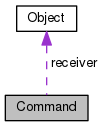
\includegraphics[width=149pt]{classCommand__coll__graph}
\end{center}
\end{figure}
\subsection*{Public Member Functions}
\begin{DoxyCompactItemize}
\item 
\hyperlink{classCommand_ab5004b23122fa06ca3613ee5d082ddc1}{Command} (\hyperlink{classObject}{Object} $\ast$new\+Receiver, \hyperlink{classCommand_a929c81cf8ef71dc52ef78156492f2a42}{Action} new\+Action)
\item 
virtual void \hyperlink{classCommand_a1f73a16e8706aec4c4db746f710b88d9}{execute} ()
\end{DoxyCompactItemize}
\subsection*{Static Public Member Functions}
\begin{DoxyCompactItemize}
\item 
static void \hyperlink{classCommand_a31a6d34a1d61f7cd994075a852714d3c}{undo} ()
\item 
static void \hyperlink{classCommand_ac807fae3326e22c02edc737708f9b288}{redo} ()
\end{DoxyCompactItemize}
\subsection*{Private Types}
\begin{DoxyCompactItemize}
\item 
typedef void(Object\+::$\ast$ \hyperlink{classCommand_a929c81cf8ef71dc52ef78156492f2a42}{Action}) ()
\end{DoxyCompactItemize}
\subsection*{Private Attributes}
\begin{DoxyCompactItemize}
\item 
\hyperlink{classObject}{Object} $\ast$ \hyperlink{classCommand_ac4a7e0c82bede3a8cd2f2b1478bd4763}{receiver}
\item 
\hyperlink{classCommand_a929c81cf8ef71dc52ef78156492f2a42}{Action} \hyperlink{classCommand_ac5473faf8b8b03ce83353838bc00c6dd}{action}
\end{DoxyCompactItemize}
\subsection*{Static Private Attributes}
\begin{DoxyCompactItemize}
\item 
static std\+::vector$<$ \hyperlink{classCommand}{Command} $\ast$ $>$ \hyperlink{classCommand_a3b694e6c1b5a3e62bdc0d7d1b3178eb1}{command\+List}
\item 
static std\+::vector$<$ \hyperlink{classMemento}{Memento} $\ast$ $>$ \hyperlink{classCommand_a03c855537275970db8e4b9c7ea64a9f9}{memento\+List}
\item 
static int \hyperlink{classCommand_a661b9cfc157529504ecf44528e4640b6}{num\+Commands} = 0
\item 
static int \hyperlink{classCommand_a06f1310ccbfdcfd18cfae03dcb428728}{max\+Commands} = 0
\end{DoxyCompactItemize}


\subsection{Member Typedef Documentation}
\index{Command@{Command}!Action@{Action}}
\index{Action@{Action}!Command@{Command}}
\subsubsection[{\texorpdfstring{Action}{Action}}]{\setlength{\rightskip}{0pt plus 5cm}typedef void(Object\+::$\ast$ Command\+::\+Action) ()\hspace{0.3cm}{\ttfamily [private]}}\hypertarget{classCommand_a929c81cf8ef71dc52ef78156492f2a42}{}\label{classCommand_a929c81cf8ef71dc52ef78156492f2a42}


\subsection{Constructor \& Destructor Documentation}
\index{Command@{Command}!Command@{Command}}
\index{Command@{Command}!Command@{Command}}
\subsubsection[{\texorpdfstring{Command(\+Object $\ast$new\+Receiver, Action new\+Action)}{Command(Object *newReceiver, Action newAction)}}]{\setlength{\rightskip}{0pt plus 5cm}Command\+::\+Command (
\begin{DoxyParamCaption}
\item[{{\bf Object} $\ast$}]{new\+Receiver, }
\item[{{\bf Action}}]{new\+Action}
\end{DoxyParamCaption}
)\hspace{0.3cm}{\ttfamily [inline]}}\hypertarget{classCommand_ab5004b23122fa06ca3613ee5d082ddc1}{}\label{classCommand_ab5004b23122fa06ca3613ee5d082ddc1}

\begin{DoxyCode}
59 : \hyperlink{classCommand_ac4a7e0c82bede3a8cd2f2b1478bd4763}{receiver} (newReceiver), \hyperlink{classCommand_ac5473faf8b8b03ce83353838bc00c6dd}{action} (newAction) \{\}
\end{DoxyCode}


\subsection{Member Function Documentation}
\index{Command@{Command}!execute@{execute}}
\index{execute@{execute}!Command@{Command}}
\subsubsection[{\texorpdfstring{execute()}{execute()}}]{\setlength{\rightskip}{0pt plus 5cm}virtual void Command\+::execute (
\begin{DoxyParamCaption}
{}
\end{DoxyParamCaption}
)\hspace{0.3cm}{\ttfamily [inline]}, {\ttfamily [virtual]}}\hypertarget{classCommand_a1f73a16e8706aec4c4db746f710b88d9}{}\label{classCommand_a1f73a16e8706aec4c4db746f710b88d9}

\begin{DoxyCode}
60                                \{
61             \textcolor{keywordflow}{if} (\hyperlink{classCommand_a03c855537275970db8e4b9c7ea64a9f9}{mementoList}.size() < \hyperlink{classCommand_a661b9cfc157529504ecf44528e4640b6}{numCommands} + 1)
62                 \hyperlink{classCommand_a03c855537275970db8e4b9c7ea64a9f9}{mementoList}.resize (\hyperlink{classCommand_a661b9cfc157529504ecf44528e4640b6}{numCommands} + 1);
63             \hyperlink{classCommand_a03c855537275970db8e4b9c7ea64a9f9}{mementoList}[\hyperlink{classCommand_a661b9cfc157529504ecf44528e4640b6}{numCommands}] = \hyperlink{classCommand_ac4a7e0c82bede3a8cd2f2b1478bd4763}{receiver}->
      \hyperlink{classObject_a169528dfd6ff33b21b038da8021cd748}{createMemento}();  \textcolor{comment}{// saves the last value}
64             \textcolor{keywordflow}{if} (\hyperlink{classCommand_a3b694e6c1b5a3e62bdc0d7d1b3178eb1}{commandList}.size() < \hyperlink{classCommand_a661b9cfc157529504ecf44528e4640b6}{numCommands} + 1)
65                 \hyperlink{classCommand_a3b694e6c1b5a3e62bdc0d7d1b3178eb1}{commandList}.resize (\hyperlink{classCommand_a661b9cfc157529504ecf44528e4640b6}{numCommands} + 1);
66             \hyperlink{classCommand_a3b694e6c1b5a3e62bdc0d7d1b3178eb1}{commandList}[\hyperlink{classCommand_a661b9cfc157529504ecf44528e4640b6}{numCommands}] = \textcolor{keyword}{this};  \textcolor{comment}{// saves the last command}
67             \textcolor{keywordflow}{if} (\hyperlink{classCommand_a661b9cfc157529504ecf44528e4640b6}{numCommands} > \hyperlink{classCommand_a06f1310ccbfdcfd18cfae03dcb428728}{maxCommands})
68                 \hyperlink{classCommand_a06f1310ccbfdcfd18cfae03dcb428728}{maxCommands} = \hyperlink{classCommand_a661b9cfc157529504ecf44528e4640b6}{numCommands};
69             \hyperlink{classCommand_a661b9cfc157529504ecf44528e4640b6}{numCommands}++;
70             (\hyperlink{classCommand_ac4a7e0c82bede3a8cd2f2b1478bd4763}{receiver}->*\hyperlink{classCommand_ac5473faf8b8b03ce83353838bc00c6dd}{action})();
71         \}
\end{DoxyCode}


Here is the call graph for this function\+:
\nopagebreak
\begin{figure}[H]
\begin{center}
\leavevmode
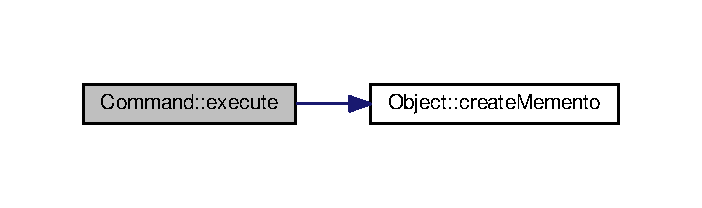
\includegraphics[width=337pt]{classCommand_a1f73a16e8706aec4c4db746f710b88d9_cgraph}
\end{center}
\end{figure}


\index{Command@{Command}!redo@{redo}}
\index{redo@{redo}!Command@{Command}}
\subsubsection[{\texorpdfstring{redo()}{redo()}}]{\setlength{\rightskip}{0pt plus 5cm}static void Command\+::redo (
\begin{DoxyParamCaption}
{}
\end{DoxyParamCaption}
)\hspace{0.3cm}{\ttfamily [inline]}, {\ttfamily [static]}}\hypertarget{classCommand_ac807fae3326e22c02edc737708f9b288}{}\label{classCommand_ac807fae3326e22c02edc737708f9b288}

\begin{DoxyCode}
81                            \{
82             \textcolor{keywordflow}{if} (\hyperlink{classCommand_a661b9cfc157529504ecf44528e4640b6}{numCommands} > \hyperlink{classCommand_a06f1310ccbfdcfd18cfae03dcb428728}{maxCommands})
83             \{
84                 std::cout << \textcolor{stringliteral}{"There is nothing to redo at this point."} << std::endl;
85                 return ;
86             \}
87             \hyperlink{classCommand}{Command}* commandRedo = \hyperlink{classCommand_a3b694e6c1b5a3e62bdc0d7d1b3178eb1}{commandList}[\hyperlink{classCommand_a661b9cfc157529504ecf44528e4640b6}{numCommands}];
88             (commandRedo->\hyperlink{classCommand_ac4a7e0c82bede3a8cd2f2b1478bd4763}{receiver}->*(commandRedo->\hyperlink{classCommand_ac5473faf8b8b03ce83353838bc00c6dd}{action}))();
89             \hyperlink{classCommand_a661b9cfc157529504ecf44528e4640b6}{numCommands}++;
90         \}
\end{DoxyCode}
\index{Command@{Command}!undo@{undo}}
\index{undo@{undo}!Command@{Command}}
\subsubsection[{\texorpdfstring{undo()}{undo()}}]{\setlength{\rightskip}{0pt plus 5cm}static void Command\+::undo (
\begin{DoxyParamCaption}
{}
\end{DoxyParamCaption}
)\hspace{0.3cm}{\ttfamily [inline]}, {\ttfamily [static]}}\hypertarget{classCommand_a31a6d34a1d61f7cd994075a852714d3c}{}\label{classCommand_a31a6d34a1d61f7cd994075a852714d3c}

\begin{DoxyCode}
72                            \{
73             \textcolor{keywordflow}{if} (\hyperlink{classCommand_a661b9cfc157529504ecf44528e4640b6}{numCommands} == 0)
74             \{
75                 std::cout << \textcolor{stringliteral}{"There is nothing to undo at this point."} << std::endl;
76                 \textcolor{keywordflow}{return};
77             \}
78             \hyperlink{classCommand_a3b694e6c1b5a3e62bdc0d7d1b3178eb1}{commandList}[\hyperlink{classCommand_a661b9cfc157529504ecf44528e4640b6}{numCommands} - 1]->receiver->reinstateMemento (
      \hyperlink{classCommand_a03c855537275970db8e4b9c7ea64a9f9}{mementoList}[\hyperlink{classCommand_a661b9cfc157529504ecf44528e4640b6}{numCommands} - 1]);
79             \hyperlink{classCommand_a661b9cfc157529504ecf44528e4640b6}{numCommands}--;
80         \}
\end{DoxyCode}


\subsection{Member Data Documentation}
\index{Command@{Command}!action@{action}}
\index{action@{action}!Command@{Command}}
\subsubsection[{\texorpdfstring{action}{action}}]{\setlength{\rightskip}{0pt plus 5cm}{\bf Action} Command\+::action\hspace{0.3cm}{\ttfamily [private]}}\hypertarget{classCommand_ac5473faf8b8b03ce83353838bc00c6dd}{}\label{classCommand_ac5473faf8b8b03ce83353838bc00c6dd}
\index{Command@{Command}!command\+List@{command\+List}}
\index{command\+List@{command\+List}!Command@{Command}}
\subsubsection[{\texorpdfstring{command\+List}{commandList}}]{\setlength{\rightskip}{0pt plus 5cm}std\+::vector$<$ {\bf Command} $\ast$ $>$ Command\+::command\+List\hspace{0.3cm}{\ttfamily [static]}, {\ttfamily [private]}}\hypertarget{classCommand_a3b694e6c1b5a3e62bdc0d7d1b3178eb1}{}\label{classCommand_a3b694e6c1b5a3e62bdc0d7d1b3178eb1}
\index{Command@{Command}!max\+Commands@{max\+Commands}}
\index{max\+Commands@{max\+Commands}!Command@{Command}}
\subsubsection[{\texorpdfstring{max\+Commands}{maxCommands}}]{\setlength{\rightskip}{0pt plus 5cm}int Command\+::max\+Commands = 0\hspace{0.3cm}{\ttfamily [static]}, {\ttfamily [private]}}\hypertarget{classCommand_a06f1310ccbfdcfd18cfae03dcb428728}{}\label{classCommand_a06f1310ccbfdcfd18cfae03dcb428728}
\index{Command@{Command}!memento\+List@{memento\+List}}
\index{memento\+List@{memento\+List}!Command@{Command}}
\subsubsection[{\texorpdfstring{memento\+List}{mementoList}}]{\setlength{\rightskip}{0pt plus 5cm}std\+::vector$<$ {\bf Memento} $\ast$ $>$ Command\+::memento\+List\hspace{0.3cm}{\ttfamily [static]}, {\ttfamily [private]}}\hypertarget{classCommand_a03c855537275970db8e4b9c7ea64a9f9}{}\label{classCommand_a03c855537275970db8e4b9c7ea64a9f9}
\index{Command@{Command}!num\+Commands@{num\+Commands}}
\index{num\+Commands@{num\+Commands}!Command@{Command}}
\subsubsection[{\texorpdfstring{num\+Commands}{numCommands}}]{\setlength{\rightskip}{0pt plus 5cm}int Command\+::num\+Commands = 0\hspace{0.3cm}{\ttfamily [static]}, {\ttfamily [private]}}\hypertarget{classCommand_a661b9cfc157529504ecf44528e4640b6}{}\label{classCommand_a661b9cfc157529504ecf44528e4640b6}
\index{Command@{Command}!receiver@{receiver}}
\index{receiver@{receiver}!Command@{Command}}
\subsubsection[{\texorpdfstring{receiver}{receiver}}]{\setlength{\rightskip}{0pt plus 5cm}{\bf Object}$\ast$ Command\+::receiver\hspace{0.3cm}{\ttfamily [private]}}\hypertarget{classCommand_ac4a7e0c82bede3a8cd2f2b1478bd4763}{}\label{classCommand_ac4a7e0c82bede3a8cd2f2b1478bd4763}


The documentation for this class was generated from the following file\+:\begin{DoxyCompactItemize}
\item 
\hyperlink{Memento_8cpp}{Memento.\+cpp}\end{DoxyCompactItemize}

\hypertarget{classFlipDownCommand}{}\section{Flip\+Down\+Command Class Reference}
\label{classFlipDownCommand}\index{Flip\+Down\+Command@{Flip\+Down\+Command}}


Inheritance diagram for Flip\+Down\+Command\+:
\nopagebreak
\begin{figure}[H]
\begin{center}
\leavevmode
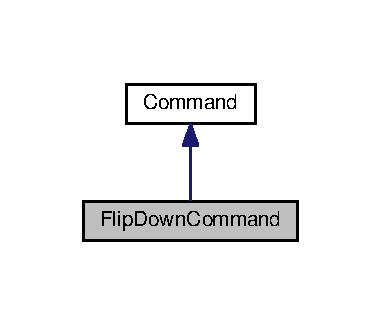
\includegraphics[width=183pt]{classFlipDownCommand__inherit__graph}
\end{center}
\end{figure}


Collaboration diagram for Flip\+Down\+Command\+:
\nopagebreak
\begin{figure}[H]
\begin{center}
\leavevmode
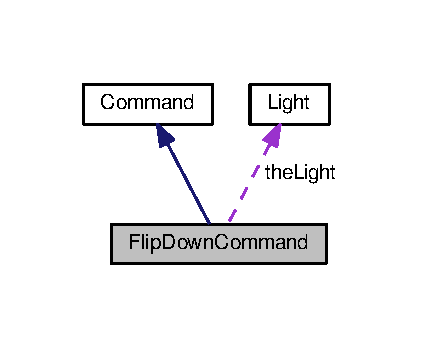
\includegraphics[width=202pt]{classFlipDownCommand__coll__graph}
\end{center}
\end{figure}
\subsection*{Public Member Functions}
\begin{DoxyCompactItemize}
\item 
\hyperlink{classFlipDownCommand_af218198d340956c93e27033f48258bf8}{Flip\+Down\+Command} (\hyperlink{classLight}{Light} \&light)
\item 
virtual void \hyperlink{classFlipDownCommand_a5514f3bdf8d7601f3252361635f9c3a1}{execute} ()
\end{DoxyCompactItemize}
\subsection*{Private Attributes}
\begin{DoxyCompactItemize}
\item 
\hyperlink{classLight}{Light} \& \hyperlink{classFlipDownCommand_a74f7f12538ecf5b5921e289a4c1129a5}{the\+Light}
\end{DoxyCompactItemize}


\subsection{Constructor \& Destructor Documentation}
\index{Flip\+Down\+Command@{Flip\+Down\+Command}!Flip\+Down\+Command@{Flip\+Down\+Command}}
\index{Flip\+Down\+Command@{Flip\+Down\+Command}!Flip\+Down\+Command@{Flip\+Down\+Command}}
\subsubsection[{\texorpdfstring{Flip\+Down\+Command(\+Light \&light)}{FlipDownCommand(Light &light)}}]{\setlength{\rightskip}{0pt plus 5cm}Flip\+Down\+Command\+::\+Flip\+Down\+Command (
\begin{DoxyParamCaption}
\item[{{\bf Light} \&}]{light}
\end{DoxyParamCaption}
)\hspace{0.3cm}{\ttfamily [inline]}}\hypertarget{classFlipDownCommand_af218198d340956c93e27033f48258bf8}{}\label{classFlipDownCommand_af218198d340956c93e27033f48258bf8}

\begin{DoxyCode}
52                                   :\hyperlink{classFlipDownCommand_a74f7f12538ecf5b5921e289a4c1129a5}{theLight}(light)
53     \{
54 
55     \}
\end{DoxyCode}


\subsection{Member Function Documentation}
\index{Flip\+Down\+Command@{Flip\+Down\+Command}!execute@{execute}}
\index{execute@{execute}!Flip\+Down\+Command@{Flip\+Down\+Command}}
\subsubsection[{\texorpdfstring{execute()}{execute()}}]{\setlength{\rightskip}{0pt plus 5cm}virtual void Flip\+Down\+Command\+::execute (
\begin{DoxyParamCaption}
{}
\end{DoxyParamCaption}
)\hspace{0.3cm}{\ttfamily [inline]}, {\ttfamily [virtual]}}\hypertarget{classFlipDownCommand_a5514f3bdf8d7601f3252361635f9c3a1}{}\label{classFlipDownCommand_a5514f3bdf8d7601f3252361635f9c3a1}


Implements \hyperlink{classCommand_a6fd7d9bd8df8bfc881e4d6c7cd1878b7}{Command}.


\begin{DoxyCode}
57     \{
58         \hyperlink{classFlipDownCommand_a74f7f12538ecf5b5921e289a4c1129a5}{theLight}.\hyperlink{classLight_aee2ab836d8c984756e10e8e301130aa4}{turnOff}();
59     \}
\end{DoxyCode}


\subsection{Member Data Documentation}
\index{Flip\+Down\+Command@{Flip\+Down\+Command}!the\+Light@{the\+Light}}
\index{the\+Light@{the\+Light}!Flip\+Down\+Command@{Flip\+Down\+Command}}
\subsubsection[{\texorpdfstring{the\+Light}{theLight}}]{\setlength{\rightskip}{0pt plus 5cm}{\bf Light}\& Flip\+Down\+Command\+::the\+Light\hspace{0.3cm}{\ttfamily [private]}}\hypertarget{classFlipDownCommand_a74f7f12538ecf5b5921e289a4c1129a5}{}\label{classFlipDownCommand_a74f7f12538ecf5b5921e289a4c1129a5}


The documentation for this class was generated from the following file\+:\begin{DoxyCompactItemize}
\item 
\hyperlink{Command_8cpp}{Command.\+cpp}\end{DoxyCompactItemize}

\hypertarget{classFlipUpCommand}{}\section{Flip\+Up\+Command Class Reference}
\label{classFlipUpCommand}\index{Flip\+Up\+Command@{Flip\+Up\+Command}}


Inheritance diagram for Flip\+Up\+Command\+:
\nopagebreak
\begin{figure}[H]
\begin{center}
\leavevmode
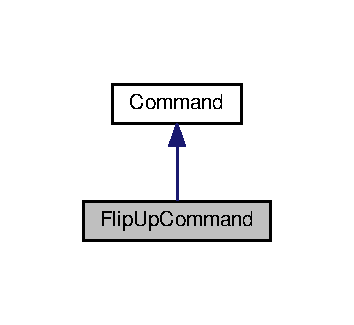
\includegraphics[width=170pt]{classFlipUpCommand__inherit__graph}
\end{center}
\end{figure}


Collaboration diagram for Flip\+Up\+Command\+:
\nopagebreak
\begin{figure}[H]
\begin{center}
\leavevmode
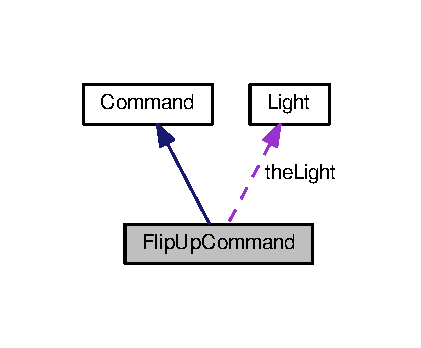
\includegraphics[width=202pt]{classFlipUpCommand__coll__graph}
\end{center}
\end{figure}
\subsection*{Public Member Functions}
\begin{DoxyCompactItemize}
\item 
\hyperlink{classFlipUpCommand_aae6e1231a8e842aa6d91843a2b2280ca}{Flip\+Up\+Command} (\hyperlink{classLight}{Light} \&light)
\item 
virtual void \hyperlink{classFlipUpCommand_a5130aaef4e36aa54f5a6a466b779b225}{execute} ()
\end{DoxyCompactItemize}
\subsection*{Private Attributes}
\begin{DoxyCompactItemize}
\item 
\hyperlink{classLight}{Light} \& \hyperlink{classFlipUpCommand_a0fbc80da677f2a8b95952585ff20b473}{the\+Light}
\end{DoxyCompactItemize}


\subsection{Constructor \& Destructor Documentation}
\index{Flip\+Up\+Command@{Flip\+Up\+Command}!Flip\+Up\+Command@{Flip\+Up\+Command}}
\index{Flip\+Up\+Command@{Flip\+Up\+Command}!Flip\+Up\+Command@{Flip\+Up\+Command}}
\subsubsection[{\texorpdfstring{Flip\+Up\+Command(\+Light \&light)}{FlipUpCommand(Light &light)}}]{\setlength{\rightskip}{0pt plus 5cm}Flip\+Up\+Command\+::\+Flip\+Up\+Command (
\begin{DoxyParamCaption}
\item[{{\bf Light} \&}]{light}
\end{DoxyParamCaption}
)\hspace{0.3cm}{\ttfamily [inline]}}\hypertarget{classFlipUpCommand_aae6e1231a8e842aa6d91843a2b2280ca}{}\label{classFlipUpCommand_aae6e1231a8e842aa6d91843a2b2280ca}

\begin{DoxyCode}
34                                :\hyperlink{classFlipUpCommand_a0fbc80da677f2a8b95952585ff20b473}{theLight}(light)
35     \{
36 
37     \}
\end{DoxyCode}


\subsection{Member Function Documentation}
\index{Flip\+Up\+Command@{Flip\+Up\+Command}!execute@{execute}}
\index{execute@{execute}!Flip\+Up\+Command@{Flip\+Up\+Command}}
\subsubsection[{\texorpdfstring{execute()}{execute()}}]{\setlength{\rightskip}{0pt plus 5cm}virtual void Flip\+Up\+Command\+::execute (
\begin{DoxyParamCaption}
{}
\end{DoxyParamCaption}
)\hspace{0.3cm}{\ttfamily [inline]}, {\ttfamily [virtual]}}\hypertarget{classFlipUpCommand_a5130aaef4e36aa54f5a6a466b779b225}{}\label{classFlipUpCommand_a5130aaef4e36aa54f5a6a466b779b225}


Implements \hyperlink{classCommand_a6fd7d9bd8df8bfc881e4d6c7cd1878b7}{Command}.


\begin{DoxyCode}
40     \{
41         \hyperlink{classFlipUpCommand_a0fbc80da677f2a8b95952585ff20b473}{theLight}.\hyperlink{classLight_a79613afb0cf7788c131091afccb46aef}{turnOn}();
42     \}
\end{DoxyCode}


\subsection{Member Data Documentation}
\index{Flip\+Up\+Command@{Flip\+Up\+Command}!the\+Light@{the\+Light}}
\index{the\+Light@{the\+Light}!Flip\+Up\+Command@{Flip\+Up\+Command}}
\subsubsection[{\texorpdfstring{the\+Light}{theLight}}]{\setlength{\rightskip}{0pt plus 5cm}{\bf Light}\& Flip\+Up\+Command\+::the\+Light\hspace{0.3cm}{\ttfamily [private]}}\hypertarget{classFlipUpCommand_a0fbc80da677f2a8b95952585ff20b473}{}\label{classFlipUpCommand_a0fbc80da677f2a8b95952585ff20b473}


The documentation for this class was generated from the following file\+:\begin{DoxyCompactItemize}
\item 
\hyperlink{Command_8cpp}{Command.\+cpp}\end{DoxyCompactItemize}

\hypertarget{classLight}{}\section{Light Class Reference}
\label{classLight}\index{Light@{Light}}
\subsection*{Public Member Functions}
\begin{DoxyCompactItemize}
\item 
\hyperlink{classLight_aeb5df09a25a32f19fdffa761268ba24f}{Light} ()
\item 
void \hyperlink{classLight_a79613afb0cf7788c131091afccb46aef}{turn\+On} ()
\item 
void \hyperlink{classLight_aee2ab836d8c984756e10e8e301130aa4}{turn\+Off} ()
\end{DoxyCompactItemize}


\subsection{Constructor \& Destructor Documentation}
\index{Light@{Light}!Light@{Light}}
\index{Light@{Light}!Light@{Light}}
\subsubsection[{\texorpdfstring{Light()}{Light()}}]{\setlength{\rightskip}{0pt plus 5cm}Light\+::\+Light (
\begin{DoxyParamCaption}
{}
\end{DoxyParamCaption}
)\hspace{0.3cm}{\ttfamily [inline]}}\hypertarget{classLight_aeb5df09a25a32f19fdffa761268ba24f}{}\label{classLight_aeb5df09a25a32f19fdffa761268ba24f}

\begin{DoxyCode}
16 \{  \}
\end{DoxyCode}


\subsection{Member Function Documentation}
\index{Light@{Light}!turn\+Off@{turn\+Off}}
\index{turn\+Off@{turn\+Off}!Light@{Light}}
\subsubsection[{\texorpdfstring{turn\+Off()}{turnOff()}}]{\setlength{\rightskip}{0pt plus 5cm}void Light\+::turn\+Off (
\begin{DoxyParamCaption}
{}
\end{DoxyParamCaption}
)\hspace{0.3cm}{\ttfamily [inline]}}\hypertarget{classLight_aee2ab836d8c984756e10e8e301130aa4}{}\label{classLight_aee2ab836d8c984756e10e8e301130aa4}

\begin{DoxyCode}
24     \{
25         cout << \textcolor{stringliteral}{"The light is off"} << endl;
26     \}
\end{DoxyCode}
\index{Light@{Light}!turn\+On@{turn\+On}}
\index{turn\+On@{turn\+On}!Light@{Light}}
\subsubsection[{\texorpdfstring{turn\+On()}{turnOn()}}]{\setlength{\rightskip}{0pt plus 5cm}void Light\+::turn\+On (
\begin{DoxyParamCaption}
{}
\end{DoxyParamCaption}
)\hspace{0.3cm}{\ttfamily [inline]}}\hypertarget{classLight_a79613afb0cf7788c131091afccb46aef}{}\label{classLight_a79613afb0cf7788c131091afccb46aef}

\begin{DoxyCode}
19     \{
20         cout << \textcolor{stringliteral}{"The light is on"} << endl;
21     \}
\end{DoxyCode}


The documentation for this class was generated from the following file\+:\begin{DoxyCompactItemize}
\item 
\hyperlink{Command_8cpp}{Command.\+cpp}\end{DoxyCompactItemize}

\hypertarget{classSwitch}{}\section{Switch Class Reference}
\label{classSwitch}\index{Switch@{Switch}}


Collaboration diagram for Switch\+:
\nopagebreak
\begin{figure}[H]
\begin{center}
\leavevmode
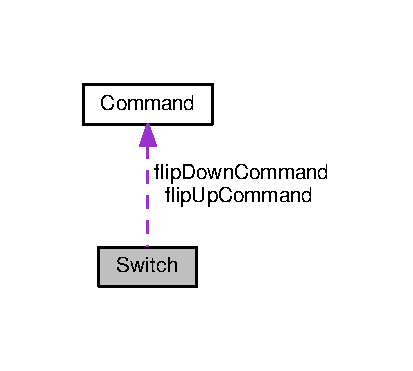
\includegraphics[width=198pt]{classSwitch__coll__graph}
\end{center}
\end{figure}
\subsection*{Public Member Functions}
\begin{DoxyCompactItemize}
\item 
\hyperlink{classSwitch_a66ba6728853f391a84ac8f9c51e25141}{Switch} (\hyperlink{classCommand}{Command} \&flip\+Up\+Cmd, \hyperlink{classCommand}{Command} \&flip\+Down\+Cmd)
\item 
void \hyperlink{classSwitch_a897907b3d656b36a8bad9a830b294504}{flip\+Up} ()
\item 
void \hyperlink{classSwitch_aa280f6f53ea293f8142f8fa2cd45c3ed}{flip\+Down} ()
\end{DoxyCompactItemize}
\subsection*{Private Attributes}
\begin{DoxyCompactItemize}
\item 
\hyperlink{classCommand}{Command} \& \hyperlink{classSwitch_aa6e2a2d4568aa542ab2e28e5a4da1d3c}{flip\+Up\+Command}
\item 
\hyperlink{classCommand}{Command} \& \hyperlink{classSwitch_af069b11fc4dab647c39da8d09edcf6c5}{flip\+Down\+Command}
\end{DoxyCompactItemize}


\subsection{Constructor \& Destructor Documentation}
\index{Switch@{Switch}!Switch@{Switch}}
\index{Switch@{Switch}!Switch@{Switch}}
\subsubsection[{\texorpdfstring{Switch(\+Command \&flip\+Up\+Cmd, Command \&flip\+Down\+Cmd)}{Switch(Command &flipUpCmd, Command &flipDownCmd)}}]{\setlength{\rightskip}{0pt plus 5cm}Switch\+::\+Switch (
\begin{DoxyParamCaption}
\item[{{\bf Command} \&}]{flip\+Up\+Cmd, }
\item[{{\bf Command} \&}]{flip\+Down\+Cmd}
\end{DoxyParamCaption}
)\hspace{0.3cm}{\ttfamily [inline]}}\hypertarget{classSwitch_a66ba6728853f391a84ac8f9c51e25141}{}\label{classSwitch_a66ba6728853f391a84ac8f9c51e25141}

\begin{DoxyCode}
67     :\hyperlink{classSwitch_aa6e2a2d4568aa542ab2e28e5a4da1d3c}{flipUpCommand}(flipUpCmd),\hyperlink{classSwitch_af069b11fc4dab647c39da8d09edcf6c5}{flipDownCommand}(flipDownCmd)
68     \{
69 
70     \}
\end{DoxyCode}


\subsection{Member Function Documentation}
\index{Switch@{Switch}!flip\+Down@{flip\+Down}}
\index{flip\+Down@{flip\+Down}!Switch@{Switch}}
\subsubsection[{\texorpdfstring{flip\+Down()}{flipDown()}}]{\setlength{\rightskip}{0pt plus 5cm}void Switch\+::flip\+Down (
\begin{DoxyParamCaption}
{}
\end{DoxyParamCaption}
)\hspace{0.3cm}{\ttfamily [inline]}}\hypertarget{classSwitch_aa280f6f53ea293f8142f8fa2cd45c3ed}{}\label{classSwitch_aa280f6f53ea293f8142f8fa2cd45c3ed}

\begin{DoxyCode}
78     \{
79         \hyperlink{classSwitch_af069b11fc4dab647c39da8d09edcf6c5}{flipDownCommand}.\hyperlink{classCommand_a6fd7d9bd8df8bfc881e4d6c7cd1878b7}{execute}();
80     \}
\end{DoxyCode}
\index{Switch@{Switch}!flip\+Up@{flip\+Up}}
\index{flip\+Up@{flip\+Up}!Switch@{Switch}}
\subsubsection[{\texorpdfstring{flip\+Up()}{flipUp()}}]{\setlength{\rightskip}{0pt plus 5cm}void Switch\+::flip\+Up (
\begin{DoxyParamCaption}
{}
\end{DoxyParamCaption}
)\hspace{0.3cm}{\ttfamily [inline]}}\hypertarget{classSwitch_a897907b3d656b36a8bad9a830b294504}{}\label{classSwitch_a897907b3d656b36a8bad9a830b294504}

\begin{DoxyCode}
73     \{
74         \hyperlink{classSwitch_aa6e2a2d4568aa542ab2e28e5a4da1d3c}{flipUpCommand}.\hyperlink{classCommand_a6fd7d9bd8df8bfc881e4d6c7cd1878b7}{execute}();
75     \}
\end{DoxyCode}


\subsection{Member Data Documentation}
\index{Switch@{Switch}!flip\+Down\+Command@{flip\+Down\+Command}}
\index{flip\+Down\+Command@{flip\+Down\+Command}!Switch@{Switch}}
\subsubsection[{\texorpdfstring{flip\+Down\+Command}{flipDownCommand}}]{\setlength{\rightskip}{0pt plus 5cm}{\bf Command}\& Switch\+::flip\+Down\+Command\hspace{0.3cm}{\ttfamily [private]}}\hypertarget{classSwitch_af069b11fc4dab647c39da8d09edcf6c5}{}\label{classSwitch_af069b11fc4dab647c39da8d09edcf6c5}
\index{Switch@{Switch}!flip\+Up\+Command@{flip\+Up\+Command}}
\index{flip\+Up\+Command@{flip\+Up\+Command}!Switch@{Switch}}
\subsubsection[{\texorpdfstring{flip\+Up\+Command}{flipUpCommand}}]{\setlength{\rightskip}{0pt plus 5cm}{\bf Command}\& Switch\+::flip\+Up\+Command\hspace{0.3cm}{\ttfamily [private]}}\hypertarget{classSwitch_aa6e2a2d4568aa542ab2e28e5a4da1d3c}{}\label{classSwitch_aa6e2a2d4568aa542ab2e28e5a4da1d3c}


The documentation for this class was generated from the following file\+:\begin{DoxyCompactItemize}
\item 
\hyperlink{Command_8cpp}{Command.\+cpp}\end{DoxyCompactItemize}

\chapter{File Documentation}
\hypertarget{Command_8cpp}{}\section{Command.\+cpp File Reference}
\label{Command_8cpp}\index{Command.\+cpp@{Command.\+cpp}}
{\ttfamily \#include $<$iostream$>$}\\*
Include dependency graph for Command.\+cpp\+:
\nopagebreak
\begin{figure}[H]
\begin{center}
\leavevmode
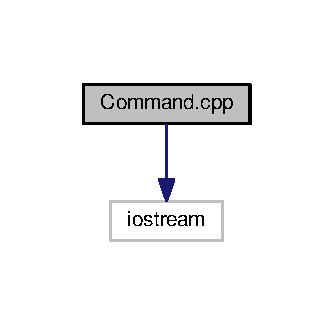
\includegraphics[width=160pt]{Command_8cpp__incl}
\end{center}
\end{figure}
\subsection*{Classes}
\begin{DoxyCompactItemize}
\item 
class \hyperlink{classCommand}{Command}
\item 
class \hyperlink{classLight}{Light}
\item 
class \hyperlink{classFlipUpCommand}{Flip\+Up\+Command}
\item 
class \hyperlink{classFlipDownCommand}{Flip\+Down\+Command}
\item 
class \hyperlink{classSwitch}{Switch}
\end{DoxyCompactItemize}
\subsection*{Functions}
\begin{DoxyCompactItemize}
\item 
int \hyperlink{Command_8cpp_ae66f6b31b5ad750f1fe042a706a4e3d4}{main} ()
\end{DoxyCompactItemize}


\subsection{Function Documentation}
\index{Command.\+cpp@{Command.\+cpp}!main@{main}}
\index{main@{main}!Command.\+cpp@{Command.\+cpp}}
\subsubsection[{\texorpdfstring{main()}{main()}}]{\setlength{\rightskip}{0pt plus 5cm}int main (
\begin{DoxyParamCaption}
{}
\end{DoxyParamCaption}
)}\hypertarget{Command_8cpp_ae66f6b31b5ad750f1fe042a706a4e3d4}{}\label{Command_8cpp_ae66f6b31b5ad750f1fe042a706a4e3d4}

\begin{DoxyCode}
90 \{
91     \hyperlink{classLight}{Light} lamp;
92     \hyperlink{classFlipUpCommand}{FlipUpCommand} switchUp(lamp);
93     \hyperlink{classFlipDownCommand}{FlipDownCommand} switchDown(lamp);
94 
95     \hyperlink{classSwitch}{Switch} s(switchUp, switchDown);
96     s.flipUp();
97     s.flipDown();
98 \}\end{DoxyCode}


Here is the call graph for this function\+:
\nopagebreak
\begin{figure}[H]
\begin{center}
\leavevmode
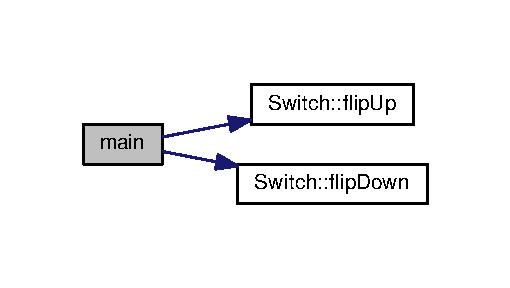
\includegraphics[width=245pt]{Command_8cpp_ae66f6b31b5ad750f1fe042a706a4e3d4_cgraph}
\end{center}
\end{figure}



%--- End generated contents ---

% Index
\backmatter
\newpage
\phantomsection
\clearemptydoublepage
\addcontentsline{toc}{chapter}{Index}
\printindex

\end{document}
